% =====================================================================
% What an SO(3) orientation flow can and cannot learn in
% molecular-crystal structure prediction
%
% Formatted for Transactions on Machine Learning Research (TMLR).
% Double-blind submission: compile with \usepackage{tmlr}. For the
% camera-ready, switch to \usepackage[accepted]{tmlr} and uncomment the
% author block below.
% Compiles standalone with tectonic / pdflatex + bibtex (tmlr.bst).
% =====================================================================
\documentclass[10pt]{article}

\usepackage{tmlr}
% \usepackage[accepted]{tmlr}   % <-- camera-ready
% \usepackage[preprint]{tmlr}   % <-- arXiv preprint

% Only standard content packages are added below; the tmlr stylefile,
% fonts, margins, and layout are left exactly as distributed.
\usepackage{amsmath,amssymb}
\usepackage{graphicx}
\usepackage{booktabs}
\usepackage{hyperref}
\usepackage{url}

\title{What an SO(3) Orientation Flow Can and Cannot Learn in\\
Molecular-Crystal Structure Prediction}

% Camera-ready author block (uncomment together with [accepted] above):
% \author{\name Frank Cai \email frankyc11223@gmail.com \\
%   \addr Purdue University, West Lafayette, IN, USA}
\author{}   % anonymized for double-blind review

\begin{document}
\maketitle

\begin{abstract}
Rigid-body factorization is an appealing route to molecular-crystal structure
prediction: freezing each molecule's conformer reduces a crystal to a lattice,
a set of fractional centroids on the torus $\mathbb{T}^3$, and a per-molecule
orientation on $\mathrm{SO}(3)$. Whether the orientation field is actually
learnable on real molecular crystals has not been examined. We introduce
SymMC-Flow, a space-group-conditioned rigid-body flow on
$\text{lattice}\times\mathbb{T}^3\times\mathrm{SO}(3)$, used as a diagnostic
study on $1{,}127$ crystals from the Cambridge Structural Database. The
lattice and centroid flows learn normally, but the absolute per-molecule
orientation flow remains at its predict-zero floor. We trace this to a
decomposition of the orientation target,
$R_m = \mathrm{rot}(g_m)\cdot R_{\text{asym}}$, into a space-group-determined
relative rotation between symmetry copies and the asymmetric unit's
gauge-arbitrary free orientation, which is not learnable from composition and
packing; the relative part is. Re-gauging to cancel the free part lifts
held-out non-reference orientation loss by $27\%$ (versus $\sim\!0\%$ for the
absolute target) and reconstructs $13.7\%$ (mean over three seeds) of
held-out multi-copy packings exactly under StructureMatcher, against $0\%$
for the predict-floor baseline. Conditioning on a discrete space-group coset
identity raises the learnable signal to roughly $48\%$ (three-seed mean),
showing the residual ceiling is set by the difficulty of \emph{inferring}
the symmetry operation from packing rather than by network capacity.
End-to-end joint generation does not yet reconstruct packings exactly,
placing this as a characterization rather than a finished generator. The
result maps what a rigid-body $\mathrm{SO}(3)$ flow can and cannot
contribute to molecular-crystal generation, and suggests such generators
should condition on crystal symmetry for the relative orientation and
sample, rather than regress, the remaining free pose.
\end{abstract}

% =====================================================================
\section{Introduction}
% =====================================================================

Crystal structure prediction (CSP) asks for the stable periodic arrangement of
a given chemical system, a problem whose combinatorial landscape has
historically demanded large ensembles of density-functional relaxations.
Generative models have emerged as a fast alternative that learns the
distribution of stable structures directly. The progression from the crystal
diffusion variational autoencoder \citep{xie2022cdvae} to joint equivariant
diffusion over lattices and fractional coordinates \citep{jiao2023diffcsp} and to
Riemannian flow matching for materials \citep{miller2024flowmm} has steadily
lowered both sample cost and error on inorganic benchmarks, where each atom is
an independent site.

Sampling cost is a practical constraint for CSP, where a single composition may
require thousands of candidate packings before relaxation and ranking. Diffusion
samplers typically integrate hundreds to a thousand steps per structure, whereas
flow matching learns a straight conditional path that off-the-shelf ordinary
differential equation solvers traverse in tens of
steps \citep{lipman2023flowmatching,chen2024riemannian}. The same advantage drove
the move from $\mathrm{SE}(3)$ diffusion to $\mathrm{SE}(3)$ flow matching for
protein backbones, where roughly five-fold fewer steps were reported at equal or
better quality \citep{yim2023se3diffusion,yim2023frameflow}. A factorized,
flow-matched generator that retains this efficiency while respecting crystal
symmetry is therefore an attractive target, provided each of its degrees of
freedom is in fact learnable.

Molecular crystals are harder. A molecular crystal couples flexible
intramolecular degrees of freedom to the rigid-body packing of whole molecules,
and the most common organic space groups place several symmetry-related copies
of a molecule in each cell, a regime where packing search has long been a
bottleneck in community blind tests \citep{price2023blindtest7} and a target for
data-efficient learned models \citep{obrien2021dataefficient}. Two design choices
have emerged. All-atom
generators predict every atomic coordinate jointly: OXtal \citep{jin2025oxtal}
learns the conditional distribution over conformation and packing with a
lattice-free diffusion model, and PackFlow \citep{subramanian2026packflow} flows
heavy-atom Cartesian coordinates and lattice parameters with a reinforcement
learning alignment step. Rigid-body generators instead treat building blocks as
rigid and predict only their pose. MOFFlow \citep{kim2025mofflow} demonstrates
this for metal--organic frameworks, casting metal nodes and organic linkers as
rigid bodies and applying $\mathrm{SE}(3)$ flow matching to their
roto-translations, which mirrors generative modeling on the rotation
group \citep{leach2022so3} and the frame-based generation developed for protein
backbones \citep{yim2023se3diffusion,yim2023frameflow}.

Rigid-body factorization is attractive for molecular crystals: it collapses
dozens of atomic coordinates per molecule to a single pose, exploits the
modularity of the cell, and supports the short sampling trajectories
characteristic of flow matching \citep{lipman2023flowmatching,chen2024riemannian}.
It also introduces a per-molecule orientation variable on the rotation group
$\mathrm{SO}(3)$. Whether that orientation field is learnable on real molecular
crystals is an open question. MOFFlow reports a working method but does not
analyze the orientation field in isolation, and the all-atom approaches sidestep
orientation altogether. No prior work asks what a rigid-body $\mathrm{SO}(3)$
orientation flow actually learns on molecular crystals, or where it fails.

This question has a classical antecedent. Established molecular-CSP codes do not
search the orientation of every symmetry copy independently; they search only
the contents of the asymmetric unit and then \emph{generate} the remaining
copies by applying the space-group operators, so the relative pose between
copies is fixed by symmetry and never a free
variable \citep{price2023blindtest7,obrien2021dataefficient}. The decomposition
we develop below is, in effect, a rediscovery of that division of labor for a
learned flow: the symmetry-relative rotation that classical search obtains for
free is what the flow can learn, and the asymmetric unit's free pose, which
classical search does sample, is what the flow cannot regress. Framing the
result this way both credits the long-standing classical practice and clarifies
why a naive per-copy orientation flow is solving a problem that symmetry already
solves in part.

This paper answers that question. We build SymMC-Flow, a
space-group-conditioned rigid-body flow on
$\text{lattice}\times\mathbb{T}^3\times\mathrm{SO}(3)$, and train it on a
corpus of $1{,}127$ molecular crystals exported from the Cambridge Structural
Database (CSD) \citep{groom2016csd}. The lattice and centroid flows learn; the
absolute per-molecule
orientation flow does not, sitting at the predict-zero floor across two corpus
sizes and after a gauge correction. We explain this with a decomposition of the
orientation target and a chain of controlled diagnostics, and we show that the
learnable component is real geometry, not a loss artifact.

Our contributions are:
\begin{itemize}
\item A rigid-body $\mathrm{SO}(3)$ flow for molecular crystals with a
molecule-intrinsic orientation gauge that removes the spurious cross-crystal
reference frame.
\item The decomposition $R_m = \mathrm{rot}(g_m)\cdot R_{\text{asym}}$ and a
falsification chain (predict-zero floor, gauge fix, scaling, clean-packing
control, relative re-gauge) that isolates the learnable symmetry-relative
orientation from the gauge-free asymmetric-unit pose.
\item An orientation-isolated StructureMatcher metric showing the learned
relative orientation reconstructs $13.7\%$ (mean over three seeds) of held-out
multi-copy packings exactly, against $0\%$ for the floor.
\item Evidence from discrete coset-identity conditioning that the residual
ceiling is inference-limited, not representational.
\end{itemize}

% =====================================================================
\section{Results}
% =====================================================================

\subsection{Rigid-body factorization and the flow}

SymMC-Flow represents a molecular crystal as a lattice $L\in\mathbb{R}^{3\times3}$,
and, for each molecule $m$, a fractional centroid $c_m\in\mathbb{T}^3$ and an
orientation $R_m\in\mathrm{SO}(3)$ acting on a shared, centered body-frame
conformer $\text{local}_m$. Atom positions follow
\begin{equation}
\text{cart}_{m,a} = c_m L + R_m\,\text{local}_{m,a},
\label{eq:factor}
\end{equation}
so every copy of a chemical species shares one conformer and differs only by its
pose. A conditional flow-matching objective \citep{lipman2023flowmatching} is
trained jointly on the three manifolds: a Euclidean path for a
volume-normalized lattice parametrization, a torus geodesic for centroids, and
an $\mathrm{SO}(3)$ geodesic for orientations, with the vector field conditioned
on the space group. An $\mathrm{E}(n)$-equivariant
encoder \citep{satorras2021egnn} embeds the conformer and pair-bias attention
mixes molecules within the cell. Architecture, manifold operations, and data
are detailed in Methods.

Each manifold is given a parametrization that makes its conditional path
well-conditioned. The lattice is not flowed as a raw $3\times3$ matrix, which
mixes scale and shape and admits negative determinants, but in a ten-dimensional
space of a per-atom log-volume and a determinant-one shape, with the prior
volume matched to the corpus mean so that the generated cells start at a
physical density. Centroids live on the periodic torus and are flowed along its
geodesics with wrap-around, so the target velocity respects the minimum-image
convention. Orientations are flowed along $\mathrm{SO}(3)$ geodesics, with the
network predicting a body-frame angular velocity and the sampler advancing by the
exponential map, which keeps every intermediate state on the manifold. This
separation matters for the analysis: the three heads can be read independently,
so a failure localized to orientation is visible against a backdrop of lattice
and centroid that train normally.

\subsection{Lattice and centroid flows learn on real molecular crystals}

The corpus is a seeded random sample of the CSD, scanning $14{,}874$ entries and
retaining $1{,}127$ ordered organic molecular crystals that factorize into
$5{,}048$ rigid blocks after the rigid-conformer and disorder gates (Methods).
We establish first that the pipeline learns the packing degrees of freedom.
Table~\ref{tab:perhead} reports the held-out per-head flow-matching loss before
and after training. The lattice loss falls by $94\%$ and the centroid loss by
$30\%$, both converging within the first epoch. The absolute orientation loss
moves by only $3.3\%$ and shows no downward trend over training. Lattice and
centroid behave as they do on inorganic benchmarks, where every block is a single
atom; orientation is the outlier, and it is the one degree of freedom that the
single-atom benchmarks never exercise.

\begin{table}[t]
\centering
\caption{Held-out per-head flow-matching loss, untrained $\rightarrow$ trained,
on the multi-copy CSD corpus under noised conditioning and a common split.
Lattice and centroid losses are independent of the orientation target; the
orientation row is the absolute target $R_m$. Lattice and centroid learn; the
absolute orientation target stays at its predict-zero floor.}
\label{tab:perhead}
\begin{tabular}{lccc}
\toprule
head & untrained & trained & change \\
\midrule
lattice            & 1.24 & 0.08 & $+94\%$ \\
centroid           & 0.36 & 0.25 & $+30\%$ \\
orientation ($R_m$)& 5.37 & 5.18 & $+3.3\%$ \\
\bottomrule
\end{tabular}
\end{table}

\subsection{The absolute orientation flow sits at a predict-zero floor}

The orientation loss equals the expected squared tangent velocity
$\mathbb{E}\lVert u_R\rVert^2\approx 5.24$ that a network outputting zero would
incur. A trained orientation head that never beats this value has learned
nothing. Three controls rule out the obvious explanations. First, the floor is
unchanged when the corpus is scaled from $250$ to $1{,}127$ crystals, so it is
not data sparsity. Second, a molecule-intrinsic orientation gauge (Methods),
which removes the arbitrary cross-crystal reference frame that would otherwise
make $R_m$ a rotation relative to some molecule in an unrelated structure, is
necessary for a well-posed target but does not lift the floor. Third, a
clean-packing control feeds the field the true (un-noised) lattice and
centroids while still noising the orientation and keeping the orientation
target, which is the best case for any two-stage scheme that generates packing
first and orientation second. Orientation still moves by only $3.3\%$
(Table~\ref{tab:twobytwo}, top row), so noised conditioning is not the cause and
a two-stage architecture cannot help. The obstruction is in the target itself.

The gauge correction deserves emphasis because it is a prerequisite for the
target to be well-posed at all. Without it, a species' body frame is set by
whichever copy is parsed first anywhere in the dataset, so $R_m$ measures
rotation relative to a molecule in an unrelated crystal, a quantity that is
random across the corpus and would floor any orientation head by construction.
Fixing the frame to a molecule-intrinsic quantity (Methods) removes this
artificial randomness, and the harder, well-posed targets it produces require a
lower learning rate to avoid an early-training divergence in the shared trunk.
With both in place the orientation head is given every chance to learn, yet the
trained loss continues to oscillate within a narrow band around the
predict-zero value with no downward trend, while lattice and centroid converge
in the same run. The failure is specific and reproducible, not an optimization
accident.

\subsection{The orientation target decomposes into a learnable and a free part}

Consider a molecule $m$ generated from an asymmetric-unit molecule by a
space-group operation with rotation part $\mathrm{rot}(g_m)$. Its absolute pose
factors as
\begin{equation}
R_m = \mathrm{rot}(g_m)\cdot R_{\text{asym}},
\label{eq:decomp}
\end{equation}
where $R_{\text{asym}}$ is the orientation of the asymmetric unit in the cell.
The first factor is determined by the space group and is shared structure across
crystals; the second is a free, per-crystal choice that dominates the target.
Because the body-frame gauge is arbitrary, $R_{\text{asym}}$ carries no
consistent training signal tied to composition or packing, which produces the
floor. The empirical distribution bears this out: the absolute reference-copy
orientations track the Haar-uniform density on $\mathrm{SO}(3)$ across the full
range of geodesic angles, with mean $122.6^\circ$ against the Haar expectation of
$126.5^\circ$ (Appendix~\ref{app:rasym}, Figure~\ref{fig:rasym}). A
Kolmogorov--Smirnov test detects only a
slight deviation from uniformity ($D=0.04$), confined to a small near-identity
excess attributable to the gauge-defining copies rather than to a broad preferred
orientation. We therefore state the claim narrowly: $R_{\text{asym}}$ is not
predictable from the conditioning available here, not that orientation is
unlearnable in principle. The distinction matters. A uniform \emph{marginal}
does not by itself establish that $R_{\text{asym}}$ is conditionally
independent of the packing; a weak dependence $p(R_{\text{asym}}\mid\text{packing})$
can coexist with a Haar marginal. Our claim is the operational one that no
exploitable signal survives our composition-and-packing conditioning. We test
this directly rather than infer it from the marginal alone: a supervised probe
trained to predict $R_{\text{asym}}$ from the lattice, the centroid arrangement,
the conformer shape, and the space group does not improve on the best
feature-free constant and sits at the no-information level
(Appendix~\ref{app:probe}), so a uniform marginal here reflects genuine conditional
unpredictability rather than masking a hidden dependence. We distinguish this
from an under-featurized model: a richer descriptor of the local environment,
such as explicit hydrogen-bond topology or dipole alignment, could in principle
expose residual signal that the present conditioning does not.

To isolate the learnable factor we re-gauge each crystal so that the first copy
of every species is a reference with $R=I$ and the remaining copies carry only
the relative rotation $R'_m = R_m R_0^{-1}$, which cancels $R_{\text{asym}}$
(Methods). The transformation leaves the reconstructed crystal unchanged. To
avoid crediting a trivial ``predict identity'' solution, we split the
orientation loss into reference copies (target $I$) and non-reference copies
(the symmetry-determined targets), and report the latter.
Table~\ref{tab:twobytwo} gives the full $2\times2$ over target and conditioning.
The absolute target floors in both conditioning regimes. The relative target
descends by $27\%$ on held-out non-reference copies and generalizes, with an
identical result under noised and clean conditioning. Across three random seeds
the non-reference drop is $27.5\pm2.7\%$ (mean $\pm$ s.d.), so the effect is
stable. Because the conformer registry is shared across crystals, a random split
could in principle let a species seen in training reappear in validation; we
therefore repeated the three-seed measurement under a stricter species-grouped
split that assigns every crystal sharing a species to the same side of the
partition (Methods). The non-reference drop is then $28.5\pm2.9\%$, statistically
indistinguishable from the random-split value, so the learnable relative signal
is not an artifact of species leakage between training and validation
(Appendix~\ref{app:grouped}). The signal therefore rides on the space group, which is conditioned
directly, together with the
coarse centroid arrangement, and is robust to conditioning noise.

The relative analysis runs on the $1{,}095$ crystals that contain at least two
copies of a species, the subset in which a non-trivial relative target exists;
their species multiplicities are dominated by two- and four-copy cells, with a
tail to sixteen. On this subset the overall orientation loss, counting both
copy classes, improves by $34$ to $36\%$, and the reference copies, whose target
is the identity, improve by $61\%$. The non-reference figure of $27\%$ is the
conservative one, since it cannot be earned by collapsing to the identity, and it
is the number we carry forward. Read together, the floor of the absolute target
and the descent of the relative target confirm Eq.~\eqref{eq:decomp}
quantitatively: the only learnable content in $R_m$ is the part that survives
cancellation of $R_{\text{asym}}$.

\begin{table}[t]
\centering
\caption{Held-out non-reference orientation loss, untrained $\rightarrow$
trained, across orientation target and conditioning. The absolute pose floors;
the relative (symmetry-determined) orientation is learnable and robust to
conditioning noise.}
\label{tab:twobytwo}
\begin{tabular}{lcc}
\toprule
target & noised conditioning & clean packing \\
\midrule
absolute $R_m$  & $5.37\!\rightarrow\!5.18$ ($+3.3\%$) & $5.35\!\rightarrow\!5.18$ ($+3.3\%$) \\
relative $R'_m$ & $5.37\!\rightarrow\!3.91$ ($+27.1\%$) & $5.37\!\rightarrow\!3.94$ ($+26.7\%$) \\
\bottomrule
\end{tabular}
\end{table}

\subsection{Relative orientation reconstructs real packings}

A drop in flow-matching loss need not correspond to correct geometry. We
therefore evaluate the learned orientation by reconstruction. Holding the true
lattice, centroid, and conformer fixed, we sample only the $\mathrm{SO}(3)$ field
and rebuild each crystal, then test whether it matches the ground truth under
pymatgen's StructureMatcher \citep{ong2013pymatgen}. The symmetry-induced relative
rotations are large, clustering near $180^\circ$ because the dominant organic
space groups, such as $P2_1/c$ and $P\bar{1}$, relate copies by two-fold
rotations and inversions \citep{groom2016csd}, so a single deterministic
integration of the field collapses to the conditional mean and underperforms. We
therefore draw eight orientation samples per crystal and take the best, the
appropriate generative read for a multimodal target. Reporting a
controlled best-of-$k$ match alongside the geodesic orientation error, rather
than a single headline rate, follows recent cautions on match-rate
metrics \citep{martirossyan2025matching}.

Table~\ref{tab:matchrate} reports the outcome on $131$ held-out multi-copy
crystals, averaged over three seeds. The oracle, which uses the true orientation,
matches every structure, confirming the metric's tolerances. The trained flow
reconstructs $13.7\pm2.0\%$ (mean $\pm$ s.d.; $12.2$, $13.0$, $16.0\%$ across
seeds) of held-out packings exactly, against $0\%$ for a random (predict-floor)
field and $0.8\%$ for the naive choice of leaving every copy un-rotated. Its mean
non-reference orientation error is $68^\circ$, below the $89^\circ$ of a random
field (Figure~\ref{fig:results}a). The $27\%$ loss reduction is real reconstructed
geometry. The reconstruction is not an artifact of the chosen tolerances:
sweeping the StructureMatcher length, site, and angle thresholds moves the rate
monotonically from $5.3\%$ at the tightest setting to $20.6\%$ at the loosest,
with the oracle matching every structure throughout, and a single deterministic
draw (match@1) still reconstructs a nonzero fraction against the $0\%$ floor
(Appendix~\ref{app:sweep}). Under the species-grouped split above, an
orientation-isolated read reconstructs $10.7\%$ of the grouped held-out crystals,
confirming the reconstruction survives the leakage control.

\begin{table}[t]
\centering
\caption{Orientation-isolated reconstruction on $131$ held-out multi-copy
crystals (true lattice, centroid, and conformer; only $\mathrm{SO}(3)$ sampled;
best of eight draws; mean over three seeds). The learned field reconstructs
packings the floor and naive baselines cannot.}
\label{tab:matchrate}
\begin{tabular}{lcc}
\toprule
condition & match rate & non-ref.\ orient.\ error \\
\midrule
oracle (true orientation) & $100.0\%$ & $0^\circ$ \\
identity (naive, $R=I$)   & $0.8\%$   & $163^\circ$ \\
untrained (predict-floor) & $0.0\%$   & $89^\circ$ \\
trained                   & $13.7\pm2.0\%$  & $68^\circ$ \\
\bottomrule
\end{tabular}
\end{table}

\subsection{The ceiling is inference-limited, not representational}

Two experiments locate the remaining gap. Increasing model capacity and
training, a wider network with more attention and encoder layers trained for more
than six times as many steps, raises the non-reference signal from $27\%$ to
$45\%$. This is real headroom, but it stops short of the $50.6\%$ reached by simply
telling the base model which symmetry coset each copy belongs to (below), an
oracle conditioning obtained without any extra capacity. Scaling the network
therefore narrows but does not close the gap, and is matched by a much smaller
model handed the discrete symmetry label; the relative target is not merely
under-fit.

The decisive test conditions the field on a discrete space-group coset identity.
For a copy generated by a crystallographic operation, the relative rotation
$R'_m$ equals that operation's rotation part, so within a space group the
non-reference relative rotations fall into a small discrete set of cosets.
Clustering the observed relative rotations by geodesic distance within each space
group yields a codebook of $707$ cosets across the corpus, and we condition each
molecule on its coset index, a discrete label of the kind used in
symmetry-conditioned crystal
generation \citep{jiao2024diffcsppp,wyckoffdiff2025,symmcd2025}, rather than the
continuous rotation itself. Table~\ref{tab:strengthen} shows that coset
conditioning raises the non-reference signal to $47.9\pm3.2\%$ over three seeds
($50.6\%$ on the single run shown in the table), with reference copies
reaching $89\%$, nearly doubling the learnable component relative to a paired
control that reproduces the $27\%$ baseline on the identical corpus and split
(Figure~\ref{fig:results}b). Most of the ceiling is therefore the difficulty of
inferring which symmetry
operation generated each copy from the noised packing, not an inability of the
$\mathrm{SO}(3)$ head to represent the rotation. The residual that remains even
with the coset supplied is attributable to the free $R_{\text{asym}}$ and to the
axial gauge freedom of symmetric-top molecules, whose orientation about a
symmetry axis is genuinely unobservable.

This experiment is a representability diagnostic, not a deployable conditioning.
Because the codebook is built by clustering the observed relative rotations, the
coset index is derived in part from the target it helps predict, so the $50.6\%$ is
an upper bound on what the discrete symmetry identity can contribute, isolating
representability from inference. The same label is in principle available at
sampling time without the answer, since the coset is a deterministic function of
the space group, the Wyckoff assignment, and the copy ordering, which
template-based generators already provide \citep{jiao2024diffcsppp,wyckoffdiff2025,symmcd2025};
realizing that gain in a sampler is left to future work.

\begin{table}[t]
\centering
\caption{Held-out non-reference orientation loss under model and conditioning
changes. Coset conditioning nearly doubles the learnable signal; the paired
control isolates the effect.}
\label{tab:strengthen}
\begin{tabular}{lcc}
\toprule
configuration & non-ref.\ loss & change \\
\midrule
baseline (relative target)        & $5.37\!\rightarrow\!3.91$ & $+27.1\%$ \\
\quad + capacity and training     & $5.42\!\rightarrow\!2.98$ & $+45.0\%$ \\
\quad + coset conditioning        & $5.36\!\rightarrow\!2.65$ & $+50.6\%$ \\
\quad coset control (no coset)    & $5.37\!\rightarrow\!3.91$ & $+27.1\%$ \\
\bottomrule
\end{tabular}
\end{table}

\begin{figure}[t]
\centering
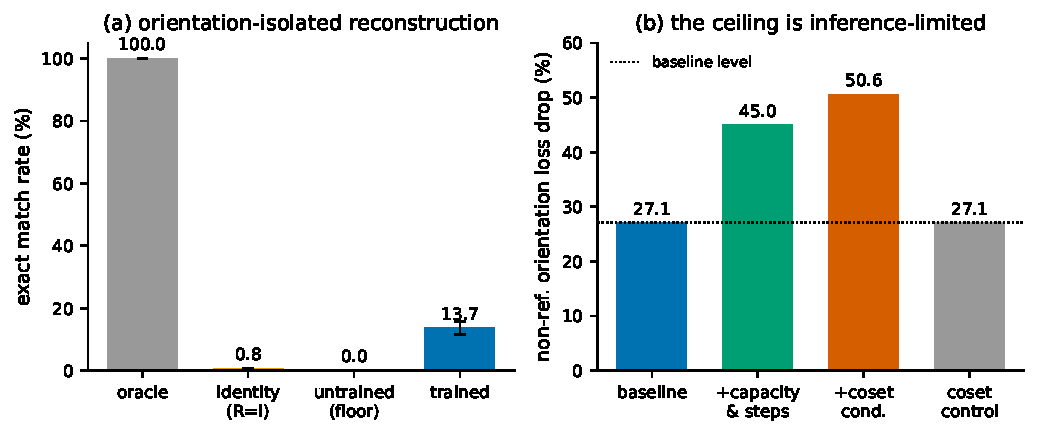
\includegraphics[width=\linewidth]{figures/fig2_results.pdf}
\caption{The orientation results. (a) Orientation-isolated StructureMatcher
reconstruction rate by condition (true lattice, centroid, and conformer; only
$\mathrm{SO}(3)$ sampled; best of eight draws; $n=131$ held-out crystals; mean
over three seeds). The trained flow reconstructs $13.7\%$ of packings exactly,
against $0\%$ for the predict-floor field and $0.8\%$ for the naive $R=I$
baseline. (b) Held-out
non-reference orientation loss drop under the strengthening levers; coset
conditioning nearly doubles the learnable signal over the baseline level (dotted),
while the no-coset control reproduces it, showing the ceiling is inference-limited
rather than representational.}
\label{fig:results}
\end{figure}

\subsection{End-to-end generation is bottlenecked by the joint packing}

The orientation-isolated metric supplies the true lattice and centroid. The
complementary question is how the full pipeline performs when all three manifolds
are sampled from the prior, that is, end-to-end rigid-body structure prediction
given only the molecular composition and conformer. Generating complete crystals
for the held-out molecules (match@20, three seeds) yields no exact match at the
StructureMatcher tolerances above ($0\%$, Wilson $95\%$ CI $0$--$2.8\%$,
$n=131$); the single-draw rate (match@1) is likewise $0\%$, so the gap is not an
artifact of the best-of-$k$ read. The best-of-$20$ per-component errors locate the
bottleneck: a median lattice-parameter error of $0.46$, a fractional centroid
error of $0.35$, and an orientation error of $57^\circ$ (medians over best-of-$20$
draws; this de-novo orientation error is not directly comparable to the
orientation-isolated $68^\circ$ of Table~\ref{tab:matchrate}, which is a mean over
best-of-$8$ draws taken with the true packing supplied). Every head contributes; in particular the
centroid field, which improves by only $30\%$ in loss, leaves molecules displaced
by roughly a third of a cell, and the orientation still carries the gauge-free
component. Scaling does not lift the joint result: the higher-capacity model
above, despite sharper components (median lattice-parameter error $0.41$,
centroid $0.35$, orientation $50^\circ$), still yields $0\%$ end-to-end at both
match@1 and match@20. To test whether this bottleneck is specific to the
rigid-body factorization or instead reflects the corpus scale, we trained an
all-atom control on the same corpus and split in which every atom is its own
block and the orientation head is disabled, the representation used by all-atom
generators \citep{jin2025oxtal,subramanian2026packflow}. Despite its lattice and
centroid heads training normally (an $88\%$ drop in flow-matching loss), it
likewise reconstructs no held-out crystal exactly (match@1 and match@20 both
$0\%$, $n=131$), equal to its own random-prior floor. Its best-of-$20$
packing-component errors are as large as the rigid-body model's (median
lattice-parameter $0.33$ and fractional-coordinate $0.46$;
Appendix~\ref{app:allatom}), locating the failure in the same joint packing. End-to-end reconstruction
at this corpus scale is therefore out of reach for the all-atom representation as
well, so the $0\%$ is a property of the scale and compute budget rather than a
deficiency unique to rigid-body factorization. This control is our own all-atom
flow trained on the same thousand-crystal corpus, not one of the published
all-atom generators \citep{jin2025oxtal,subramanian2026packflow}, which are trained
on far larger datasets with substantially more compute; the comparison therefore
shows that the all-atom \emph{representation at this scale} does not rescue
end-to-end generation, not that those larger models would fail. The
orientation-isolated $13.7\%$ is therefore an upper bound that is attainable only
when the packing is supplied, and end-to-end molecular-crystal generation at this
corpus scale and compute budget remains open. This is consistent with the scope
of the paper: the contribution is the characterization of the orientation field,
not a finished generator.

\subsection{Method validation on inorganic benchmarks}

For completeness we validated the SymMC-Flow architecture on standard
single-block inorganic benchmarks, where orientation is inactive. On carbon-24
and MP-20 the method is competitive with joint equivariant
diffusion \citep{jiao2023diffcsp} at roughly an order of magnitude fewer sampling
steps, winning some match cells and losing others. Full numbers and the
head-to-head protocol are given in Appendix~\ref{app:inorganic}; these results
confirm the flow and sampler are sound and are not the focus of this study.

% =====================================================================
\section{Discussion}
% =====================================================================

The orientation field of a rigid-body molecular-crystal flow is neither fully
learnable nor uniformly broken. It splits into a space-group-determined relative
orientation that a flow learns and reconstructs, and a gauge-free
asymmetric-unit orientation that the model cannot predict from composition and
packing. This split is a property of the representation, not of the optimizer or
the architecture, which is why it survives gauge correction, data scaling,
capacity increases, and clean conditioning.

The decomposition reconciles the divergent design choices in the field. All-atom
generators \citep{jin2025oxtal,subramanian2026packflow} never expose
$R_{\text{asym}}$ as an explicit target and so do not encounter the floor,
trading the low dimensionality of the rigid-body representation for a target
without a gauge obstruction. MOFFlow \citep{kim2025mofflow} succeeds with a
rigid-body $\mathrm{SE}(3)$ flow in part because framework connectivity
constrains block orientations far more tightly than the free pose of a molecule
in a van der Waals packing, shrinking the gauge-free component. The present
analysis predicts that rigid-body $\mathrm{SO}(3)$ generation will be most
effective precisely where orientation is constrained by the surrounding network
or by high site symmetry, and least effective for low-symmetry organic packings.

On evaluation, the gap between the flat orientation loss and the $13.7\%$
reconstruction rate shows why a single match-rate number is an unreliable
summary \citep{martirossyan2025matching}: the learnable signal is visible only
when the metric isolates orientation and samples the multimodal target. We
report the geodesic error and a controlled best-of-$k$ match for this reason.

The coset result also carries a practical implication for how rigid-body
generators should be conditioned. Template-based pipelines already supply a
space group and Wyckoff assignment at sampling time, and the coset index is a
deterministic function of that assignment together with the copy ordering. A
generator that consumes this discrete label, as space-group- and
Wyckoff-conditioned models already do for atomic
sites \citep{jiao2024diffcsppp,wyckoffdiff2025,symmcd2025}, converts the
inference-limited part of the orientation field into a near-deterministic
lookup, leaving only the free pose to be sampled. This suggests that
the right division of labor for rigid-body molecular CSP is to condition on
symmetry for the relative orientation and to sample, rather than regress, the
remaining gauge-free degree of freedom.

This study has limits. End-to-end generation does not yet reconstruct held-out
packings exactly, and the analysis isolates orientation rather than delivering a
finished generator. A de-novo stable--unique--novel evaluation would not add much
here either, because the universal interatomic potentials used to judge stability
are trained on inorganic data \citep{deng2023chgnet} and do not transfer to organic
molecular crystals; we therefore evaluate by reconstruction against known
structures. The corpus is roughly one thousand crystals and training is at modest
scale, so the absolute generation numbers should be read as a lower bound that
more data and compute would improve. The rigid-conformer gate excludes flexible
molecules by construction, and the conformer registry is shared across crystals,
so a species whose conformer differs between polymorphs beyond tolerance is
rejected. The corpus is therefore one of rigid, largely organic
(C/H/N/O-dominated) molecules, and the conclusions should be read with that
scope. The unlearnability statement is likewise scoped to molecules on
\emph{general} positions, where the asymmetric-unit pose is genuinely free; a
molecule sitting on a special position carries a site symmetry that constrains
its orientation, and that constraint is in principle learnable, consistent with
the prediction above that rigid-body $\mathrm{SO}(3)$ generation is most useful
where site symmetry is high. These choices keep the rigid-body benchmark honest
but narrow its coverage.

Two directions follow. A hybrid that predicts a rigid pose and then refines the
conformer would extend the approach to flexible molecules while keeping the
fast pose flow. Conditioning the orientation field on Wyckoff or coset
information at sampling time, suggested by the coset experiment, would convert
the inference-limited component into a usable signal whenever the symmetry
assignment is available, as it is in template-based generation.

% =====================================================================
\section{Methods}
% =====================================================================

\subsection{Rigid-body factorization and intrinsic gauge}
Each crystal is parsed into rigid molecular blocks by a covalent-bond graph with
periodic-boundary unwrapping. Molecules of one species are keyed by a
Weisfeiler--Lehman hash of the element-labelled bond graph and share a single
reference conformer; atom correspondence between a copy and its reference is the
minimum-RMSD graph isomorphism, so a molecule's own automorphisms inject no
spurious rotation. The reference conformer is rotated into a molecule-intrinsic
frame given by the principal axes of its gyration tensor, with per-axis sign
fixed by an element-weighted third moment and the frame forced right-handed.
This removes the arbitrary cross-crystal reference that otherwise makes $R_m$ a
rotation relative to an unrelated molecule, the gauge correction referenced in
Results. The pose $R_m$ of each copy is then the Kabsch rotation aligning it to
the intrinsic frame. Lattices are rebuilt from their six cell parameters to a
canonical frame.

\subsection{Manifolds and flow matching}
The lattice is flowed in a ten-dimensional parametrization of per-atom
log-volume and a determinant-one shape, with a straight-line conditional path.
Centroids follow torus geodesics; orientations follow $\mathrm{SO}(3)$
geodesics with the tangent velocity as target. We use conditional flow
matching \citep{lipman2023flowmatching} with optimal-transport coupling of the
exchangeable prior and data within each crystal \citep{pooladian2023multisample}.
Sampling integrates the field from the prior to the data manifold with a
deterministic Runge--Kutta scheme, using the $\mathrm{SO}(3)$ exponential map
for the orientation update; molecular-crystal samples used here take fifty
steps, approximately $0.26$~s per structure on a single RTX 5090 GPU in batches
of $32$, consistent with the order-of-magnitude step-count reduction that
motivates flow matching over diffusion. The construction follows Riemannian flow
matching \citep{chen2024riemannian} and parallels frame-based generative models
for proteins \citep{yim2023se3diffusion,yim2023frameflow} and metal--organic
frameworks \citep{kim2025mofflow}. The orientation target is the constant-velocity
geodesic tangent $u_R = \log(R_0^\top R_1)$ carried in the body frame, where
$R_0$ is the prior and $R_1$ the data orientation, and the loss is the squared
geodesic residual between the predicted and target tangents averaged over real
molecules.

\subsection{Predict-zero floor and clean-packing control}
The predict-zero floor is the loss of the trivial field that outputs the zero
velocity, $\mathbb{E}\lVert u_R\rVert^2$, estimated by averaging the squared
target tangent over the validation set; it is the value a head must beat to have
learned anything, and on this corpus it is approximately $5.24$. The
clean-packing control replaces the noised conditioning state with the true
lattice and centroids while leaving the orientation input noised and the
orientation target unchanged, so no label information leaks. Under this control
the lattice and centroid heads see a state inconsistent with their own velocity
targets and their losses are not interpretable, which is why only the orientation
number is read from that run.

\subsection{Network}
An $\mathrm{E}(n)$-equivariant graph network \citep{satorras2021egnn} encodes each
conformer into an invariant token. Tokens are augmented with the current
centroid, orientation, lattice, time, and a space-group embedding, then mixed by
pair-bias attention with pairwise features built from torus and Cartesian
displacements. Three heads predict the lattice, centroid, and orientation
velocities. The centroid field can be symmetrized over the space-group action.
For the coset experiment a per-molecule coset embedding is added to each token
when enabled.

\subsection{Relative gauge and coset codebook}
The relative gauge sets the first copy of each species to $R=I$ and replaces the
others by $R'_m = R_m R_0^{-1}$, with the shared conformer transformed by
$R_0$ so that reconstruction is unchanged; a reference mask records which copies
are trivial. The coset codebook clusters non-reference relative rotations within
each space group by geodesic distance into a shared set of discrete indices,
which become the per-molecule coset labels.

\subsection{Training}
Models are trained with Adam at a learning rate of $3\times10^{-4}$, gradient
clipping, and a batch size of $16$. The reduced learning rate, relative to a
common default of $10^{-3}$, is needed because the intrinsic-frame orientation
targets produce larger early gradients that otherwise diverge in the shared
trunk within the first tens of steps. The lattice prior volume per atom is
matched to the corpus mean so that generated cells begin at a physical density.
Held-out losses are averaged over several independent draws of the flow time and
prior at a fixed seed, so that the untrained and trained measurements are taken
under identical random conditions and their difference reflects learning rather
than sampling noise. The baseline relative run uses the default network
($d{=}128$, four attention layers, four encoder layers) for $800$ steps; the
capacity run widens the model to $d{=}256$ with six attention and five encoder
layers and trains for $5{,}000$ steps. A non-finite-step guard skips any
optimizer update whose loss or gradient norm is not finite, so a transient
ill-conditioned batch in the higher-capacity model cannot corrupt the weights;
the run reported here skipped a single step.

\subsection{Species-grouped split and all-atom baseline}
The species-grouped split guards against leakage from the shared conformer
registry. We build an undirected graph whose nodes are crystals and whose edges
join any two crystals that share a chemical species, take its connected
components by union--find, and assign whole components to training or validation,
so no species appears on both sides. The relative-orientation diagnostic is then
rerun over three split seeds at the default network and batch size and compared to
the random-split result. The all-atom baseline replaces the rigid-body
factorization with one block per atom and disables the orientation head
($\lambda_{\text{orient}}=0$), matching the all-atom representation; it is trained
on the same corpus and split and evaluated for de-novo reconstruction against both
its random-prior floor and the trained field.

\subsection{Orientation-isolated match metric}
Reconstruction holds the true lattice, centroid, and conformer fixed and
integrates only the orientation field from a random $\mathrm{SO}(3)$ prior under
clean-packing conditioning. Reconstructed crystals are built with
Eq.~\eqref{eq:factor} and compared to the ground truth with
StructureMatcher \citep{ong2013pymatgen} using a length tolerance of $0.3$, a site
tolerance of $0.5$, and an angle tolerance of $10^\circ$, slightly looser than
the pymatgen defaults to accommodate the rebuilt cells. The oracle row, which
reconstructs every structure at these tolerances, confirms they are not so loose
as to admit spurious matches. For each crystal we draw eight orientation samples
and count a match if any draw matches; we also report the minimum mean geodesic
error over draws on non-reference copies. Reported match rates carry a binomial
(Wilson) $95\%$ confidence interval of approximately $\pm6$ percentage points at
$n=131$.

\subsection{Data}
The corpus is a seeded random sample of the CSD (database version 601, accessed
via the CSD Python API) \citep{groom2016csd} filtered to ordered, organic,
three-dimensional, non-polymeric molecular crystals within size and
$Z'$ bounds, yielding $1{,}127$ crystals and $5{,}048$ rigid blocks from
$14{,}874$ scanned entries; $1{,}095$ contain at least two copies of a species
and define the multi-copy subset used for the relative and coset analyses. The
species multiplicities of that subset are concentrated at two and four copies
per cell, with smaller populations at three, six, eight, twelve, and sixteen,
reflecting the general-position multiplicities of the common organic space
groups. A fixed seed gives a $964/131$ train/validation split, used identically
across every diagnostic so that comparisons are paired. CSD structures are not
redistributable; a refcode manifest and the export and analysis code reproduce
the dataset from a licensed CSD installation (see the Reproducibility Statement).

% =====================================================================
\section*{Reproducibility Statement}
% =====================================================================
All architectural, manifold, training, and evaluation details needed to
reproduce the diagnostics are specified in Methods and Appendices
\ref{app:inorganic}--\ref{app:allatom}: the flow-matching objective and
$\mathrm{SO}(3)$/torus/lattice manifold operations, the intrinsic-gauge and
relative-gauge constructions, the coset codebook, the network, the Adam
hyperparameters and step budgets, the species-grouped split, and the
StructureMatcher tolerances used for the orientation-isolated metric.

The molecular-crystal corpus is a seeded random sample of the Cambridge
Structural Database (CSD) \citep{groom2016csd}. The CSD is licence-restricted, so
the CIF structures and the factorized tensors derived from them cannot be
redistributed; this is the sole reason the primary data are not openly deposited.
Reproduction on any licensed CSD installation is nonetheless fully determined: a
manifest of the $3{,}500$ CSD refcodes used to build the corpus, together with
per-entry selection metadata (formula, $Z'$, R-factor, atom count, and space
group), and the export and factorization scripts, deterministically regenerate
the exact corpus and derived tensors, and a fixed random seed reproduces the
identical $964/131$ train/validation split used throughout. The complete
SymMC-Flow implementation, the data-preparation pipeline, and this refcode
manifest will be released in a public repository and permanently archived upon
publication; they are withheld from this submission only to preserve
double-blind anonymity, and an anonymized copy can be provided to reviewers
through the OpenReview discussion on request.

The authors used an AI coding and writing assistant for software development and
manuscript copy-editing; all scientific claims, experiments, and results were
verified by the authors, who take full responsibility for the content.

% =====================================================================
\section*{Broader Impact Statement}
% =====================================================================
This is a diagnostic study of what a generative flow can and cannot learn about
molecular-crystal packing. It advances basic methodology for predicting crystal
structures from molecular composition, a capability relevant to computational
chemistry and materials discovery, including the screening of candidate
polymorphs of organic solids. The work reports a characterization rather than a
deployable generator, introduces no new released datasets, and builds no system
that acts on people or that presents an evident dual-use risk; we therefore
foresee no negative societal impact specific to this work beyond those broadly
associated with accelerating molecular and materials design. All experiments use
structures from a licensed crystallographic database under its terms of use.

\bibliographystyle{tmlr}
\bibliography{references}

% =====================================================================
\appendix
% =====================================================================
\renewcommand{\thetable}{A\arabic{table}}
\renewcommand{\thefigure}{A\arabic{figure}}
% Keep hyperref anchors unique after resetting the visible counters,
% so appendix Table A1 does not collide with main-text Table 1.
\renewcommand{\theHtable}{app.table.\arabic{table}}
\renewcommand{\theHfigure}{app.figure.\arabic{figure}}
\setcounter{table}{0}
\setcounter{figure}{0}

% ---------------------------------------------------------------------
\section{Method validation on single-block inorganic benchmarks}
\label{app:inorganic}
% ---------------------------------------------------------------------

The orientation analysis in the main text isolates a target obstruction that is
specific to multi-copy molecular crystals. To confirm that the underlying
SymMC-Flow architecture, training objective, and Runge--Kutta sampler are sound
independently of that obstruction, we benchmarked the model on two standard
single-block datasets, carbon-24 and MP-20, in which each atom is its own rigid
block and the orientation head is inactive ($\lambda_{\text{orient}}=0$). These
results are reported for completeness; they are not the contribution of this
paper.

\paragraph{Protocol.} We compare against joint equivariant
diffusion \citep{jiao2023diffcsp} using its released models, with matched
evaluation: $256$ held-out targets, $20$ samples per target, and the same
root-mean-square structure distance routine for both methods. Match rate at $k$
(``match@$k$'') is the fraction of targets for which at least one of $k$ samples
matches the reference under StructureMatcher \citep{ong2013pymatgen}. SymMC-Flow
samples in $50$ Runge--Kutta steps, against roughly $1{,}000$ steps for the
diffusion baseline.

\paragraph{Outcome.} Table~\ref{tab:inorganic} shows a mixed result: each method
wins two of the four match cells. SymMC-Flow leads on carbon-24 match@1 and on
MP-20 match@20, while the diffusion baseline leads on MP-20 match@1 and on
carbon-24 match@20 and produces tighter RMSE on matched structures. The honest
summary is that SymMC-Flow is competitive at roughly an order of magnitude fewer
sampling steps, not a uniform improvement. This is sufficient to establish that
the flow and sampler are well-behaved, which is all the main-text analysis
requires.

\begin{table}[h]
\centering
\caption{SymMC-Flow versus a diffusion baseline \citep{jiao2023diffcsp} on
single-block inorganic CSP under a matched evaluation ($256$ targets, $20$
samples, identical RMSD routine). Match rates in percent; higher is better. Each
method wins two of the four cells.}
\label{tab:inorganic}
\begin{tabular}{llcc}
\toprule
dataset & metric & SymMC-Flow & diffusion baseline \\
\midrule
carbon-24 & match@1  & \textbf{26.7} & 18.8 \\
carbon-24 & match@20 & 79.7 & \textbf{89.1} \\
MP-20     & match@1  & 41.4 & \textbf{48.0} \\
MP-20     & match@20 & \textbf{80.5} & 76.2 \\
\bottomrule
\end{tabular}
\end{table}

\paragraph{Caveat on benchmarks.} Recent work shows that carbon-24 contains a
large fraction of duplicate structures and that match-rate metrics can mislead
when identical building blocks exhibit structural
variety \citep{martirossyan2025matching}. The numbers above should be read as a
sanity check on the architecture under the field's conventional protocol rather
than as a definitive ranking.

% ---------------------------------------------------------------------
\section{Is the absolute molecular orientation uniform on SO(3)?}
\label{app:rasym}
% ---------------------------------------------------------------------

The main-text claim that the free asymmetric-unit pose $R_{\text{asym}}$ carries
no learnable signal predicts that the absolute per-molecule orientations should be
close to Haar-uniform on $\mathrm{SO}(3)$, since a uniform target offers nothing to
predict. For Haar-uniform rotations the geodesic angle $\theta$ from the identity
has density $p(\theta)=(1-\cos\theta)/\pi$ on $[0,\pi]$, with mean $126.5^\circ$.
Figure~\ref{fig:rasym} compares the empirical distribution of the reference-copy
orientations, which equal $R_{\text{asym}}$ up to the operation generating the
first-detected copy, to this density. The empirical distribution tracks the Haar
curve across the full angular range, with mean $122.6^\circ$ ($n=1{,}467$). A
one-sample Kolmogorov--Smirnov test against the Haar law gives $D=0.04$, a small
but nonzero deviation localized to a near-identity excess that comes from the
gauge-defining copies, whose self-alignment lands near the identity. The absolute
orientation is therefore close to uniform, consistent with the predict-zero floor,
and the residual deviation is a gauge artifact rather than a broad packing
preference.

\begin{figure}[h]
\centering
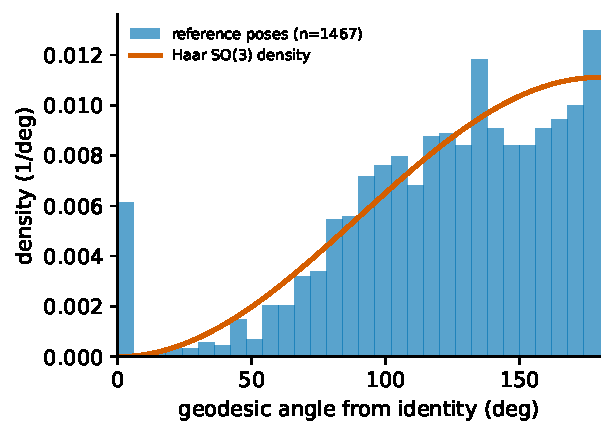
\includegraphics[width=0.62\linewidth]{figures/figS_rasym.pdf}
\caption{Empirical distribution of absolute reference-copy orientations (geodesic
angle from the identity) against the Haar-uniform $\mathrm{SO}(3)$ density. The two
agree across the range apart from a small near-identity excess from gauge-defining
copies.}
\label{fig:rasym}
\end{figure}

% ---------------------------------------------------------------------
\section{Is \texorpdfstring{$R_{\text{asym}}$}{R\_asym} conditionally predictable from packing?}
\label{app:probe}
% ---------------------------------------------------------------------

The uniformity test of the previous section concerns the \emph{marginal}
distribution of $R_{\text{asym}}$. A uniform marginal is necessary but not
sufficient for the operational claim that packing carries no signal about the
free pose: a weak conditional dependence
$p(R_{\text{asym}}\mid\text{packing})$ can coexist with a Haar marginal once the
packing is marginalized out. We therefore test the conditional directly with a
supervised probe. For each species we form a feature vector from the lattice cell
parameters, the molecule's fractional centroid, the mean and spread of all
centroids in the cell, the conformer's intrinsic shape (the gyration-tensor
eigenvalues), the molecule and atom counts, and a learned space-group embedding,
and we train a three-layer network to regress the reference-copy orientation
(a continuous six-dimensional rotation parametrization with a Frobenius loss).
The probe sees only composition and packing; the orientation is never an input.

Table~\ref{tab:probe} reports the held-out geodesic error against two references:
the single best feature-free predictor, which is the Fr\'echet (chordal) mean of
the training orientations, and a random-rotation guess. Averaged over three
splits the probe attains $125.2^\circ$, which does not improve on the
feature-free constant at $122.4^\circ$ and is statistically indistinguishable from
the random-guess level of $123.5^\circ$; the probe's mean ``improvement'' over the
constant is $-2.4\%$, i.e.\ no improvement. The network can drive its training
error well below these values, so the failure is one of generalization, not of
capacity. The conditional test thus reaches the same conclusion as the marginal
one by an independent route: under the composition-and-packing conditioning
available here, $R_{\text{asym}}$ is not predictable, which is the precise,
operational sense in which we call it unlearnable.

\begin{table}[h]
\centering
\caption{Conditional-predictability probe for $R_{\text{asym}}$: held-out mean
geodesic error (degrees, mean over three splits; lower is better). The probe,
given composition and packing, does not beat the feature-free constant and sits
at the no-information level.}
\label{tab:probe}
\begin{tabular}{lc}
\toprule
predictor & held-out geodesic error \\
\midrule
random guess (no information)        & $123.5^\circ$ \\
constant (Fr\'echet mean, feature-free) & $122.4^\circ$ \\
probe (composition + packing features)  & $125.2^\circ$ \\
\bottomrule
\end{tabular}
\end{table}

% ---------------------------------------------------------------------
\section{StructureMatcher tolerance sweep for the orientation-isolated rate}
\label{app:sweep}
% ---------------------------------------------------------------------

The main-text reconstruction rate uses a length tolerance of $0.3$, a site
tolerance of $0.5$, and an angle tolerance of $10^\circ$. To show the result is
not an artifact of that choice, Table~\ref{tab:sweep} sweeps the three
StructureMatcher tolerances on a representative trained checkpoint, reporting both
a single deterministic draw (match@1) and the best of eight draws (match@8). The
match decision uses \texttt{StructureMatcher.fit} (maximum atomic displacement
$\leq$ the site tolerance), the same strict criterion as the headline; the median
root-mean-square displacement is computed only over structures that already pass.
The rate rises monotonically from $5.3\%$ at the tightest setting to $20.6\%$ at
the loosest, while the oracle that uses the true orientation matches every
structure at all four settings, confirming the tolerances are not so loose as to
admit spurious matches. The default row ($0.3/0.5/10^\circ$) gives $16.0\%$
match@8 on this checkpoint; the main-text $13.7\pm2.0\%$ is the mean over three
independent training seeds at this row.

\begin{table}[h]
\centering
\caption{Orientation-isolated reconstruction under a StructureMatcher tolerance
sweep (single trained checkpoint; $n=131$ held-out multi-copy crystals; true
lattice, centroid, and conformer; only $\mathrm{SO}(3)$ sampled). The oracle
matches every structure at every setting. Match decided by
\texttt{StructureMatcher.fit}; RMSD is over matched structures only.}
\label{tab:sweep}
\begin{tabular}{ccccccc}
\toprule
$\ell$tol & stol & angle & match@1 & match@8 & med.\ RMSD (\AA) & oracle match@8 \\
\midrule
0.20 & 0.20 & $8^\circ$  & $0.0\%$ & $5.3\%$  & $0.089$ & $100\%$ \\
0.30 & 0.30 & $10^\circ$ & $1.5\%$ & $9.9\%$  & $0.113$ & $100\%$ \\
0.30 & 0.50 & $10^\circ$ & $3.8\%$ & $16.0\%$ & $0.128$ & $100\%$ \\
0.50 & 0.70 & $15^\circ$ & $4.6\%$ & $20.6\%$ & $0.142$ & $100\%$ \\
\bottomrule
\end{tabular}
\end{table}

% ---------------------------------------------------------------------
\section{Leakage-controlled species-grouped split}
\label{app:grouped}
% ---------------------------------------------------------------------

Because a single conformer registry is shared across crystals, a random
train/validation split could place two crystals of the same species on opposite
sides, raising the concern that the learnable relative-orientation signal reflects
species memorization rather than transferable geometry. We rule this out with a
species-grouped split (Methods): crystals sharing any species are grouped by
union--find and whole groups are assigned to one side, so no species crosses the
partition. Table~\ref{tab:grouped} compares the held-out non-reference
orientation drop under the two split regimes over three seeds. The grouped split
gives $28.5\pm2.9\%$, statistically indistinguishable from the random-split
$27.5\pm2.7\%$, so the effect is not species leakage. An orientation-isolated
reconstruction read on the grouped split (seed 0) recovers $10.7\%$ of held-out
crystals (match@8; $4.6\%$ match@1; median RMSD $0.140$~\AA) against $0\%$ for the
predict-floor field, confirming the reconstruction also survives the leakage
control.

\begin{table}[h]
\centering
\caption{Held-out non-reference orientation drop under random versus
species-grouped train/validation splits (three seeds each, mean $\pm$ s.d.). The
grouped split eliminates shared-species overlap; the signal is unchanged.}
\label{tab:grouped}
\begin{tabular}{lc}
\toprule
split & non-reference drop \\
\midrule
random (main text)        & $27.5\pm2.7\%$ \\
species-grouped (no leakage) & $28.5\pm2.9\%$ \\
\bottomrule
\end{tabular}
\end{table}

% ---------------------------------------------------------------------
\section{All-atom de-novo baseline}
\label{app:allatom}
% ---------------------------------------------------------------------

To place the $0\%$ end-to-end rigid-body result in context, we trained an
all-atom control that discards the rigid-body factorization: every atom is its own
block and the orientation head is disabled ($\lambda_{\text{orient}}=0$), the
representation used by all-atom molecular-crystal
generators \citep{jin2025oxtal,subramanian2026packflow}. It is trained on the same
$964/131$ split and evaluated for de-novo reconstruction (all manifolds sampled
from the prior) against both a random-prior floor and the trained field, with
match@20 best-of-twenty draws. Its lattice and centroid heads train normally (an
$88\%$ drop in flow-matching loss over $8{,}000$ steps), yet it reconstructs no
held-out crystal exactly: match@1 and match@20 are both $0\%$ (Wilson $95\%$ CI
$0$--$2.8\%$, $n=131$), identical to the random-prior floor
(Table~\ref{tab:allatom}). End-to-end molecular-crystal reconstruction at this
corpus scale is therefore out of reach for the all-atom representation as well, so
the $0\%$ reported for rigid-body generation reflects the corpus scale and compute
budget rather than a deficiency unique to the rigid-body factorization. This is
our own all-atom flow at the thousand-crystal scale, not one of the published
all-atom generators \citep{jin2025oxtal,subramanian2026packflow} trained on far
larger corpora; it isolates the effect of the representation at a fixed scale and
makes no claim about those larger models.

The best-of-twenty packing-component errors confirm the failure is the same joint
packing that bottlenecks the rigid-body model, not a representation-specific
pathology: the trained all-atom flow leaves a median lattice-parameter error of
$0.33$ and a median fractional-coordinate error of $0.46$ (Table~\ref{tab:allatom}),
comparable to the rigid-body de-novo errors reported in the main text (lattice
$0.46$, centroid $0.35$). Both representations place molecules roughly a third to a
half of a cell from their true positions, which is why neither reconstructs a
crystal exactly.

\begin{table}[h]
\centering
\caption{De-novo all-atom reconstruction on $131$ held-out crystals (all manifolds
sampled, best of twenty draws). The trained all-atom flow does not beat its
random-prior floor at this corpus scale, despite its packing heads training
normally, and its best-of-twenty packing errors match the rigid-body model's.}
\label{tab:allatom}
\begin{tabular}{lcccc}
\toprule
field & match@1 & match@20 & med.\ lattice-param & med.\ frac.\ coord. \\
\midrule
random prior (floor)   & $0.0\%$ & $0.0\%$ & --- & --- \\
trained all-atom flow  & $0.0\%$ & $0.0\%$ & $0.33$ & $0.46$ \\
\bottomrule
\end{tabular}
\end{table}

\end{document}
